\begin{figure}[ht]
	\centering
	\footnotesize

	\psfrag{x}[c][c] {$x$}
	\psfrag{y}[c][c] {$y$}

	\psfrag{n}[c][c] {$\Bn$}
	\psfrag{u}[c][c] {$\Bnu$}

	\psfrag{p}[c][c] {$+$}
	\psfrag{m}[c][c] {$-$}

	\psfrag{e}[c][c] {$\varepsilon$}
	\psfrag{R}[c][c] {$R$}
	\psfrag{O}[c][c] {$\mathcal{O}$}

	\psfrag{pBR}[c][c] {$\partial B_{R}(0)$}
	\psfrag{pBe}[c][c] {$\partial B_{\varepsilon}(0)$}

	\psfrag{oe}[l][l] {$\Omega_{\varepsilon} := B_R(0) \setminus B_\varepsilon (0) $}
	\psfrag{Be}[l][l] {$B_\varepsilon (0) $}
	\psfrag{BR}[l][l] {$B_R(0)$}

	\psfrag{bd}[c][c] {$\varphi(\Bx)\Big|_{\partial B_{R}(0)} = 0, \
		\forall \varphi\in \mathcal{C}^{\infty}_{0}(\mathbb{R}^2) $}

	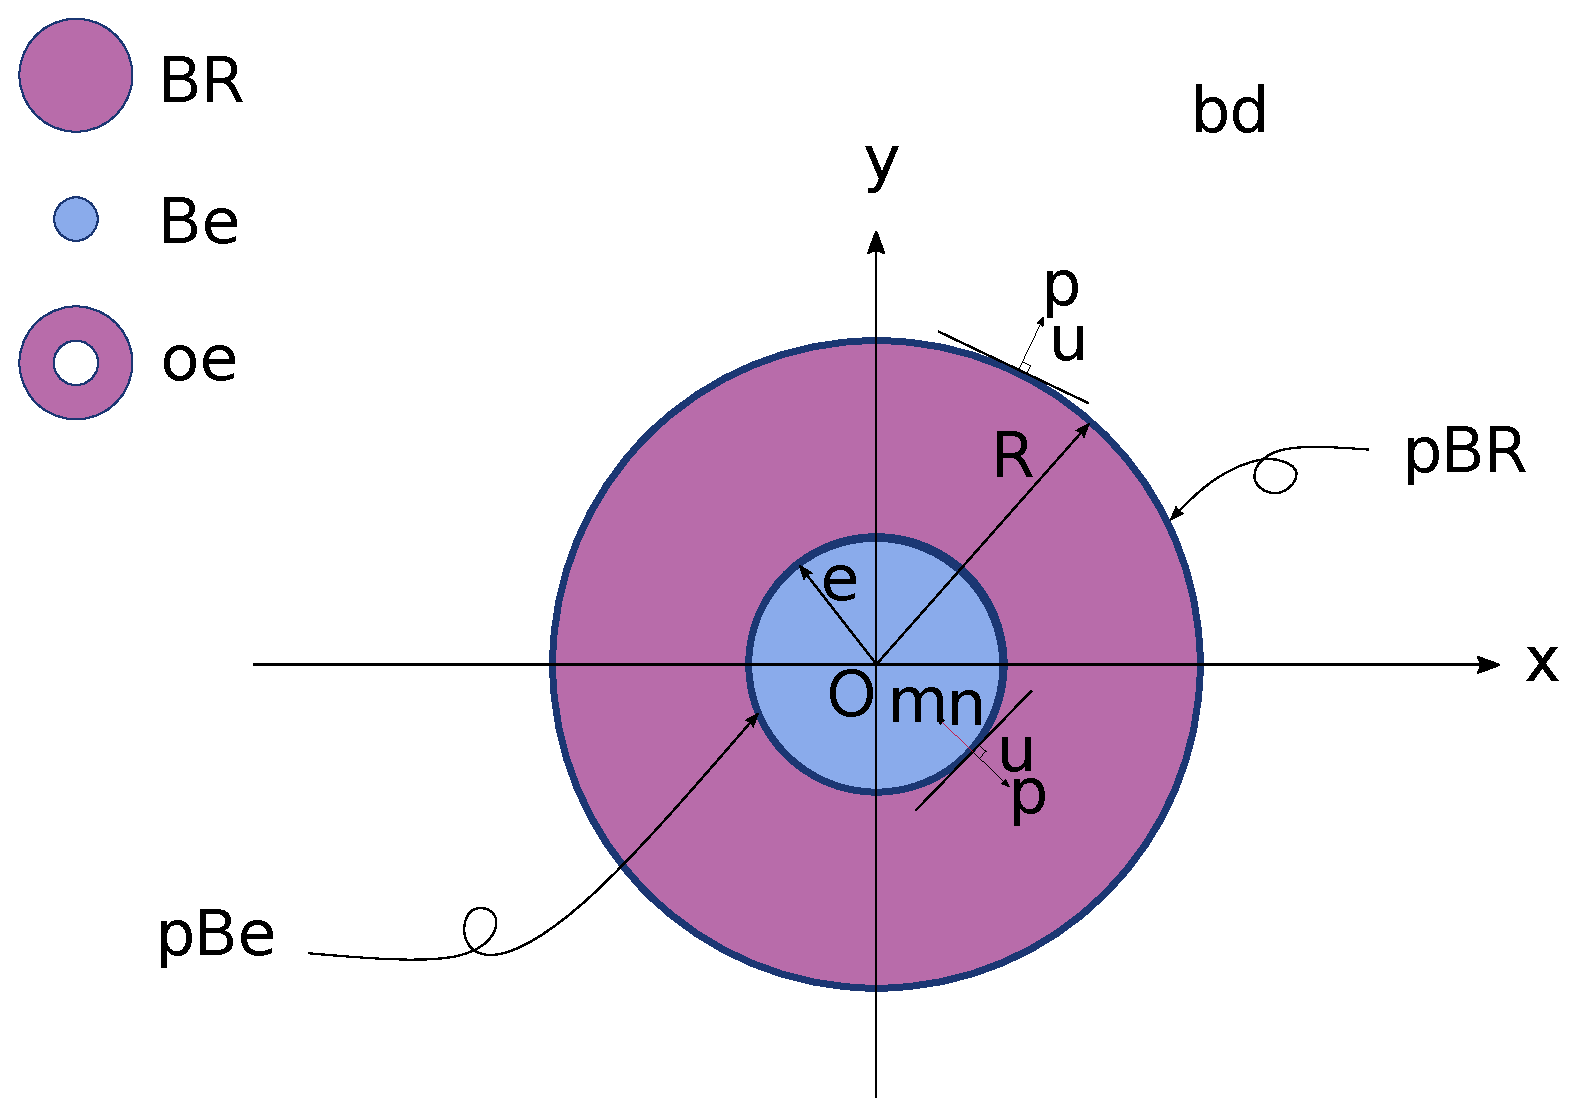
\includegraphics[width=0.8\textwidth]{ballBRBe.eps}
	\caption{The \textit{2D doughnut}: $\Omega_{\varepsilon} = B_R(0) \setminus B_\varepsilon (0) $.}
	\label{\LABEL}
\end{figure}